\documentclass[10pt,a4paper,UTF8]{article}
\usepackage{zclorg}
\author{zcl.space}
\date{}
\title{有限回溯长度的Viterbi译码器}
\hypersetup{
 pdfauthor={zcl.space},
 pdftitle={有限回溯长度的Viterbi译码器},
 pdfkeywords={communication viterbi ECC},
 pdfsubject={为了节约译码器内存,通常将译码器的回溯长度设定为约束长度的5倍左右。本文简单介绍回溯长度有限的Viterbi译码器及其性能},
 pdfcreator={Emacs 25.0.50.1 (Org mode 8.3.3)}, 
 pdflang={English}}
\begin{document}

\maketitle
\tableofcontents


\section{引言}
\label{sec:orgheadline1}


在《\href{ECCviterbi.org}{卷积编码和Viterbi译码}》 一文的最后一节,有两个问题,其中一个问:当卷积编码器的码块输入变得越来越长时,译码回溯长度也增大,为保存幸存路径所需要的内存随着回溯长度呈指数增长,怎么办? 一个有效的解决办法是:限制回溯长度。实验证明,当Viterbi译码器的回溯长度为编码器约束长度的5倍时就不会带来性能的损失。本文对此做简单的验证分析。

本文的编码器与《\href{ECCviterbi.org}{卷积编码和Viterbi译码}》 一文中的编码器保持一致:约束长度为3,生成多项式为 \([7,5]_{8}\) ,码率为 \(1/2\)。编码结束时,本文依然对编码器做清零操作(上了厕所要记得冲,:), flushing the encoer)。对于带自动冲洗功能的卷积编码器,倘若输入二进制比特序列长度为 \(N\),约束长度为 \(K\),码率为 \(1/2\)则编码输出长度为 \(2N+ 2(K-1)\),其中 \(2(K-1)\)个编码比特就是冲洗编码器产生的额外输出。
\section{Viterbi译码过程回顾}
\label{sec:orgheadline2}


在介绍有限回溯长度的Viterbi译码器之前,我们先简要回顾Viterbi译码过程,分四步:

\begin{enumerate}
\item 在接收端,一次输入两个接收比特给译码器。这两个比特可能是星座图判决的硬输出(硬比特),也可能是星座图判决的软输出(软比特)。针对这两个接收比特,计算汉明距离(应比特)或者欧式距离(软比特)。
\item 对于篱笆图中的四个状态,计算路径度量(path metric)。在计算这四个状态的路径度量时,每一个状态都有两个父状态(即,可以从两个状态到达当前状态)。对于每一个可能条状态跳转,计算其路径度量,加上之前的路径度量,得到当前路径的度量。然后,选择一条较小路径度量的路径作为幸存路径。这就是Viterbi译码过程中的加比选过程。
\item 保存当前状态幸存路径上的前一个状态。
\item 当处理\(2N+ 2(K-1)\)个比特之后,我们知道卷积编码器的状态是00(这就是在编码的时候对编码器进行清零的好处)。我们就从00状态开始回溯。我们在第2步和第3步已经保存了所有幸存路径的前后状态。根据前后状态的改变,我们很容易就得到输入比特。这些输入比特就是Viterbi译码输出。
\end{enumerate}

在进行第4步时,我们需要 \(2^{K-1}\times (N+k-1)\)个内存单元保存幸存状态矩阵。 \textbf{当 \(N\)变得很大时} ,需要大量的内存,实在不符合低复杂度接收机的原则。有没有办法降低Viterbi译码器对内存的需求,同时保证译码器性能不降低?答案是:有。

\section{有限回溯长度的Viterbi译码器}
\label{sec:orgheadline3}


通常,我把有限回溯长度的Viterbi译码器叫做“两步一回头”译码器。两步的大小分别是译码长度和纯粹回溯长度,一回头是指走完两步后就回溯译码。现在,你可能还不是很明白到底什么是“两步一回头”。看图\ref{fig:orgparagraph1}

\begin{figure}[htb]
\centering
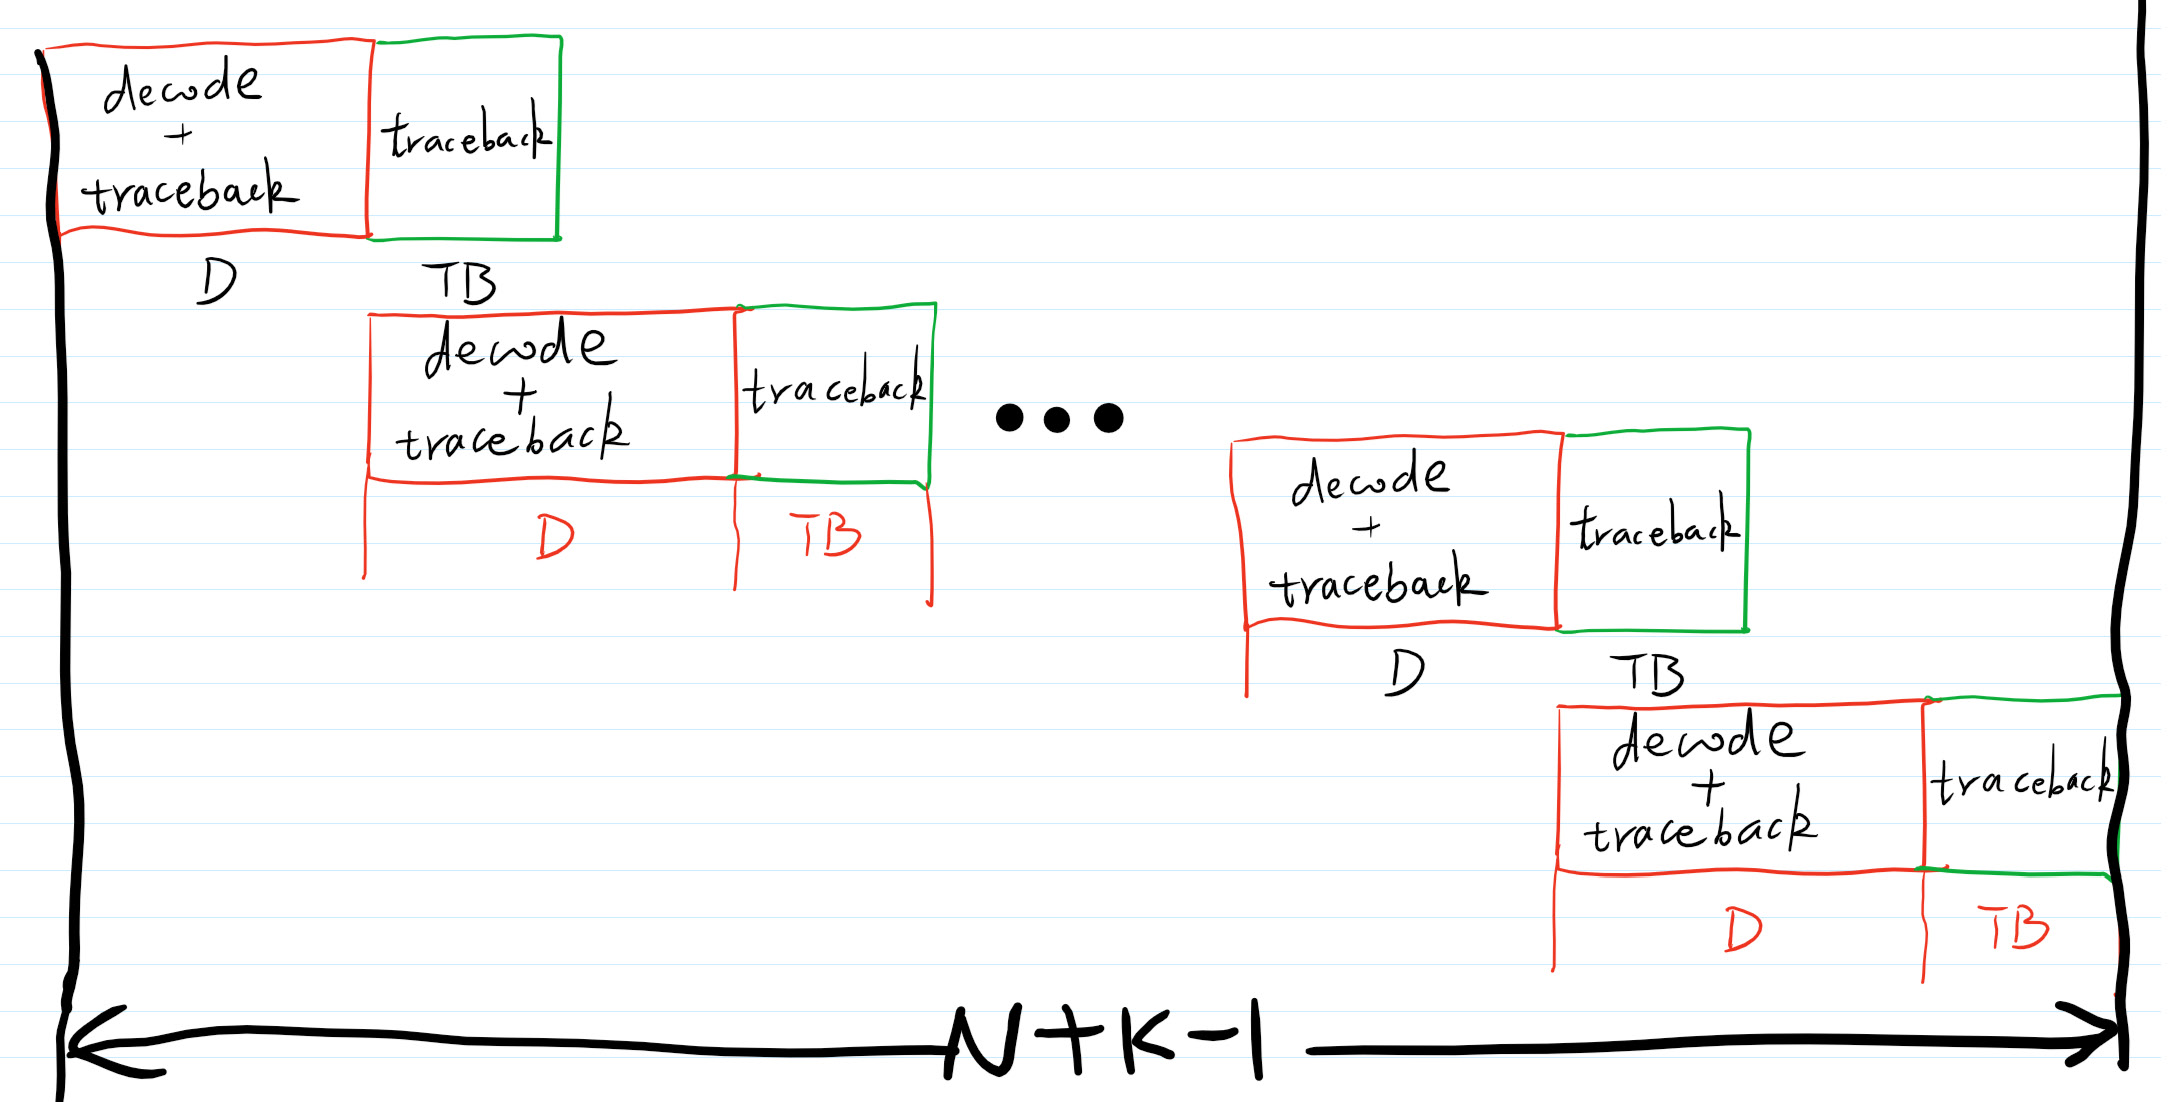
\includegraphics[width=0.6\textwidth]{../../img/20160117ViterbiFiniteTracebackLength.jpg}
\caption{\label{fig:orgparagraph1}
“两步一回头”有限回溯长度的Viterbi译码器}
\end{figure}

在图\ref{fig:orgparagraph1}中,总长为 \(N+K-1\)长的篱笆图倍分成多段,每段长度为 \(D+TB\), 在译码过程中,每处理 \(2*(D+TB)\) 长度的接收比特(对应长度为  \(D+TB\) 的信息比特,记住我们的卷积编码码率为1/2.) 回溯 \(TB\)长度,然后开始译码,译码长度为 \(D\)。依次类推,直到译出长度为 \(N+K-1\)的信息序列。整个过程可以总结为:

\begin{enumerate}
\item 在 \(D+TB\) 时刻,开始回溯。在当前的幸存路径上回溯 \(TB\)次之后,开始译码,译码长度为 \(D\)。
\item 在 \(2D+TB\) 时刻,再次开始回溯。在当前的幸存路径上回溯 \(TB\)次之后,开始译码,译码长度为 \(D\)。
\item 依次类推,直到 \(N+K-1\),我们知道篱笆图的最终状态为00,再次回溯译码。
\end{enumerate}

注意在每\(D+TB\) 的幸存路径加比选过程中,都执行Viterbi算法。在图\ref{fig:orgparagraph1}所示的译码算法过程中,只需要 \(D+2TB\)内存。另外,回溯过程中,初始状态的选择也很关键,通常有两种选择:

\begin{enumerate}
\item 总是从一个固定状态回溯(比如固定从00状态)。
\item 从最小度量的状态开始。
\end{enumerate}

实验表明,无论从那种状态回溯,当回溯长度大于5倍的约束长度时,性能无差别。对于本文的译码器,回溯长度为15已经看不出有什么区别。
\end{document}
